\documentclass[11pt,a4paper]{article}

% ------------------------------------------------------------------------------
% Encoding, Fonts, and Typography
% ------------------------------------------------------------------------------
\usepackage[utf8]{inputenc}
\usepackage[T1]{fontenc}
\usepackage{lmodern}
\usepackage{microtype}

% ------------------------------------------------------------------------------
% Geometry and Page Layout
% ------------------------------------------------------------------------------
\usepackage[margin=2.2cm,headheight=15pt,footskip=12mm]{geometry}
\usepackage{fancyhdr}
\usepackage{lastpage}

% ------------------------------------------------------------------------------
% Mathematics and Symbols
% ------------------------------------------------------------------------------
\usepackage{amsmath,amssymb,amsfonts,amsthm,mathtools}

% ------------------------------------------------------------------------------
% Tables, Arrays, and Graphics
% ------------------------------------------------------------------------------
\usepackage{booktabs}
\usepackage{tabularx}
\usepackage{multirow}
\usepackage{array}
\usepackage{graphicx}
\usepackage{colortbl}

% ------------------------------------------------------------------------------
% Colors and Boxes
% ------------------------------------------------------------------------------
\usepackage{xcolor}
\usepackage[most]{tcolorbox}

\definecolor{primary}{RGB}{24, 43, 73}       % Deep Polito Navy
\definecolor{secondary}{RGB}{38, 93, 114}    % Steel Slate Blue
\definecolor{codebg}{RGB}{248, 249, 250}     % Code background
\definecolor{boxbg}{RGB}{245, 248, 252}      % Soft question box background
\definecolor{solbg}{RGB}{240, 250, 245}      % Soft solution box background
\definecolor{solborder}{RGB}{46, 125, 50}    % Forest Green for solutions
\definecolor{alertred}{RGB}{198, 40, 40}     % Red for penalties/errors
\definecolor{highlightgreen}{RGB}{220, 245, 220} % Highlight for table

% ------------------------------------------------------------------------------
% Listings (Code Syntax Highlighting)
% ------------------------------------------------------------------------------
\usepackage{listings}

\lstdefinestyle{pythonstyle}{
    backgroundcolor=\color{codebg},
    commentstyle=\color{gray!80!black}\itshape,
    keywordstyle=\color{primary}\bfseries,
    numberstyle=\tiny\color{gray},
    stringstyle=\color{secondary!80!black},
    basicstyle=\ttfamily\footnotesize,
    breakatwhitespace=false,
    breaklines=true,
    captionpos=b,
    keepspaces=true,
    numbers=left,
    numbersep=7pt,
    showspaces=false,
    showstringspaces=false,
    showtabs=false,
    tabsize=4,
    frame=single,
    rulecolor=\color{gray!30},
    xleftmargin=12pt,
    framexleftmargin=6pt
}

\lstdefinestyle{diffstyle}{
    backgroundcolor=\color{codebg},
    basicstyle=\ttfamily\footnotesize,
    breaklines=true,
    numbers=none,
    frame=single,
    rulecolor=\color{gray!30}
}

% ------------------------------------------------------------------------------
% Lists and Enumerations
% ------------------------------------------------------------------------------
\usepackage{enumitem}
\setlist{nosep}

% ------------------------------------------------------------------------------
% Hyperlinks and Metadata
% ------------------------------------------------------------------------------
\usepackage{hyperref}
\hypersetup{
    colorlinks=true,
    linkcolor=primary,
    citecolor=secondary,
    urlcolor=secondary,
    pdftitle={Exam 2025-02-11: Large Language Models for Software Engineering},
    pdfauthor={Politecnico di Torino}
}

% ------------------------------------------------------------------------------
% Custom Question and Solution Environments
% ------------------------------------------------------------------------------
\newtcolorbox{questionbox}[2][]{
    enhanced,
    breakable,
    colback=boxbg,
    colframe=primary,
    fonttitle=\bfseries\sffamily\color{white},
    title={#2},
    arc=2.5mm,
    boxrule=1pt,
    left=9pt,
    right=9pt,
    top=7pt,
    bottom=7pt,
    before skip=10pt,
    after skip=10pt,
    #1
}

\newtcolorbox{solutionbox}[2][]{
    enhanced,
    breakable,
    colback=solbg,
    colframe=solborder,
    fonttitle=\bfseries\sffamily\color{white},
    title={#2},
    arc=2.5mm,
    boxrule=1.2pt,
    left=9pt,
    right=9pt,
    top=7pt,
    bottom=7pt,
    before skip=12pt,
    after skip=14pt,
    #1
}

\newtcolorbox{takeawaybox}[1][Key Takeaways]{
    enhanced,
    colback=white,
    colframe=secondary,
    fonttitle=\bfseries\sffamily\color{white},
    title={#1},
    arc=1.5mm,
    boxrule=0.8pt,
    left=7pt,
    right=7pt,
    top=5pt,
    bottom=5pt,
    before skip=6pt,
    after skip=6pt
}

% ------------------------------------------------------------------------------
% Header and Footer Style
% ------------------------------------------------------------------------------
\pagestyle{fancy}
\fancyhf{}
\fancyhead[L]{\small\textsc{LLMs for Software Engineering} -- Politecnico di Torino}
\fancyhead[R]{\small\textbf{Exam: 2025-02-11}}
\fancyfoot[C]{\small Page \thepage\ of \pageref{LastPage}}
\renewcommand{\headrulewidth}{0.5pt}
\renewcommand{\footrulewidth}{0.3pt}

% ------------------------------------------------------------------------------
% Document Content
% ------------------------------------------------------------------------------
\begin{document}

% --- Header Title Block ---
\begin{center}
    {\Large\textbf{\color{primary}POLITECNICO DI TORINO}}\\[3pt]
    {\large Master of Science in Computer Engineering / Data Science}\\[4pt]
    {\Large\textbf{\color{secondary}Large Language Models (Large Language Models for Software Engineering)}}\\[6pt]
    \textbf{Official Examination Session -- February 11, 2025}\\[2pt]
    \small Duration: 75 minutes (14:11 -- 15:26) \quad$\vert$\quad Total Available Points: 18.00 \quad$\vert$\quad Number of Questions: 12
\end{center}
\vspace{-4pt}
\hrule height 1.2pt
\vspace{12pt}

% --- Summary Metadata Box ---
\noindent
\begin{tcolorbox}[colback=white,colframe=primary!70,arc=1.5mm,boxrule=0.7pt,left=8pt,right=8pt,top=6pt,bottom=6pt]
\footnotesize
\textbf{Instructions to Candidates:}
\begin{itemize}[leftmargin=1.5em]
    \item The examination consists of 12 questions spanning foundational language modeling, transformer mechanics, agentic workflows, quantization, and software engineering evaluation metrics.
    \item Carefully note penalty rules: questions with penalties subtract $25\%$ of the question's base score per incorrect choice. Questions marked with ``no penalty'' do not penalize incorrect attempts.
    \item In Part I, the complete, unabridged exam questions as presented to students are recorded.
    \item In Part II, comprehensive, production-grade solutions, mathematical derivations, error diagnoses, and theoretical commentaries are provided.
\end{itemize}
\end{tcolorbox}

\vspace{10pt}

% ==============================================================================
\section{Part I: Exam Questions}
% ==============================================================================

% ------------------------------------------------------------------------------
% Question 1
% ------------------------------------------------------------------------------
\begin{questionbox}{Question 1 \hfill [2.00 Points $\vert$ No Penalty]}
What is the likely output of the following code snippet?
\begin{center}
Provide a brief explanation (max 50 words).\\
If an error occurs, indicate the line number and briefly explain why.
\end{center}

\begin{lstlisting}[style=pythonstyle]
from transformers import AutoModel, AutoTokenizer

model_name = "bert-base-uncased"
model = AutoModel.from_pretrained(model_name)
tokenizer = AutoTokenizer.from_pretrained(model_name)

prompt = "The result of the operation 2 + 2 is "
tokens = tokenizer(prompt, return_tensors="pt")

result = model.generate(**tokens)
print(tokenizer.batch_decode(result))
\end{lstlisting}

\begin{center}
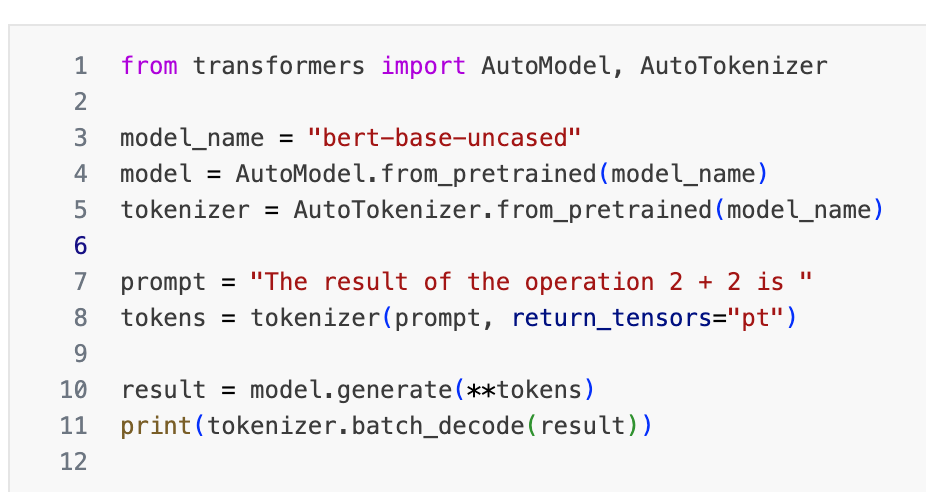
\includegraphics[width=0.72\textwidth]{assets/page_1_img_0.png}
\end{center}
\end{questionbox}

% ------------------------------------------------------------------------------
% Question 2
% ------------------------------------------------------------------------------
\begin{questionbox}{Question 2 \hfill [1.00 Point $\vert$ Penalty: $-0.25$ Points]}
What is the purpose of reflection in an agentic system?
\begin{enumerate}[label=\alph*.,leftmargin=2em]
    \item To eliminate the need for structured workflows
    \item To generate human-like responses using predefined scripts
    \item To store knowledge permanently in short-term memory
    \item To execute tasks without modifying strategies
    \item To evaluate past decisions and improve future performance
\end{enumerate}
\end{questionbox}

% ------------------------------------------------------------------------------
% Question 3
% ------------------------------------------------------------------------------
\begin{questionbox}{Question 3 \hfill [1.00 Point $\vert$ Penalty: $-0.25$ Points]}
What is the main difference between encoder-decoder cross-attention and encoder self-attention?
\begin{enumerate}[label=\alph*.,leftmargin=2em]
    \item In encoder-decoder cross-attention, the decoder attends only to the current token in the input sequence, while in encoder self-attention, the encoder attends to all tokens in the input
    \item Encoder self-attention attends to the encoder's output, while encoder-decoder cross-attention attends to the decoder's previous tokens
    \item In encoder self-attention, the decoder attends to the input sequence, whereas in encoder-decoder cross-attention, the encoder attends to the output sequence
    \item Encoder self-attention is used in the decoder, and encoder-decoder cross-attention is used in the encoder
    \item None of the other options is correct
    \item Encoder-decoder cross-attention attends only to the previous tokens in the output sequence, while encoder self-attention attends only to tokens in the input sequence
    \item Encoder self-attention only uses information from the input sequence, while encoder-decoder cross-attention allows the decoder to attend to the encoder's output
\end{enumerate}
\end{questionbox}

% ------------------------------------------------------------------------------
% Question 4
% ------------------------------------------------------------------------------
\begin{questionbox}{Question 4 \hfill [1.50 Points $\vert$ No Penalty]}
You are given the following sequence of characters:
\begin{center}
\texttt{a c e a c e a a a a a c b}
\end{center}
Initially, each character is a separate token.\\
Apply Byte-Pair Encoding (BPE) to produce 3 additional tokens. What are the generated tokens?\\
Write each token, in the correct order, in the following slots.\\
Separate the merged tokens with a comma (and no spaces).

\medskip
\noindent
\textbf{Examples:}
\begin{itemize}[leftmargin=1.5em]
    \item 1) If the merged tokens are \texttt{aa} and \texttt{b}, write: \texttt{aa,b}
    \item 2) If the merged tokens are \texttt{x} and \texttt{y}, write: \texttt{x,y}
\end{itemize}

\medskip
\begin{tabular}{ll}
\textbf{1st merge:} & \underline{\hspace{4cm}} \\
\textbf{2nd merge:} & \underline{\hspace{4cm}} \\
\textbf{3rd merge:} & \underline{\hspace{4cm}} \\
\end{tabular}
\end{questionbox}

% ------------------------------------------------------------------------------
% Question 5
% ------------------------------------------------------------------------------
\begin{questionbox}{Question 5 \hfill [1.00 Point $\vert$ Penalty: $-0.25$ Points]}
Which of the following best describes how BERTScore evaluates text similarity?
\begin{enumerate}[label=\alph*.,leftmargin=2em]
    \item It measures sequence similarity using $n$-gram co-occurrence weighted by IDF scores
    \item It uses a fine-tuned BERT model to classify whether the reference and candidate texts are semantically related or not
    \item It predicts a similarity score by treating the evaluation task as a masked language modeling problem, where BERT predicts the score as the next token
    \item It assigns similarity scores based on syntactic parse trees rather than token embeddings
    \item It uses cosine similarity on static word embeddings trained with Word2Vec or GloVe
    \item It applies a bag-of-words model to compare token frequency distributions between reference and candidate texts
    \item It computes token-level similarity by aligning contextualized embeddings from a pre-trained transformer model and aggregating scores
\end{enumerate}
\end{questionbox}

% ------------------------------------------------------------------------------
% Question 6
% ------------------------------------------------------------------------------
\begin{questionbox}{Question 6 \hfill [2.00 Points $\vert$ No Penalty]}
Apply \textbf{absmax quantization} to the following values $x_1, x_2, x_3, x_4$, to map them to signed 8-bit integers (\texttt{int8}):
\begin{align*}
    x_1 &= -5 \\
    x_2 &= 4 \\
    x_3 &= -1 \\
    x_4 &= 0
\end{align*}
Write the quantized integer versions in the following boxes:
\begin{align*}
    \text{quantized}(x_1) &= \underline{\hspace{3cm}} \\
    \text{quantized}(x_2) &= \underline{\hspace{3cm}} \\
    \text{quantized}(x_3) &= \underline{\hspace{3cm}} \\
    \text{quantized}(x_4) &= \underline{\hspace{3cm}}
\end{align*}
\end{questionbox}

% ------------------------------------------------------------------------------
% Question 7
% ------------------------------------------------------------------------------
\begin{questionbox}{Question 7 \hfill [1.00 Point $\vert$ Penalty: $-0.25$ Points per wrong selection]}
Which of the following are benefits of using open-source datasets for training LLMs?
\begin{enumerate}[label=\alph*.,leftmargin=2em]
    \item Authenticity and credibility of real-world data
    \item Guaranteed high accuracy in model predictions
    \item Ability to acquire timely data and share data freely
    \item Elimination of bias in training data
    \item LLMs no longer require fine-tuning
\end{enumerate}
\end{questionbox}

% ------------------------------------------------------------------------------
% Question 8
% ------------------------------------------------------------------------------
\begin{questionbox}{Question 8 \hfill [3.00 Points $\vert$ No Penalty]}
Consider a scenario where you have:
\begin{itemize}[leftmargin=1.5em]
    \item A natural language description of a function's requirements (\texttt{REQS})
    \item A set of test cases (\texttt{TESTS}) specifying expected inputs and outputs
\end{itemize}
You need to design an agentic architecture using LLaMA-based agents to:
\begin{enumerate}[label=\arabic*.,leftmargin=1.5em]
    \item Generate an initial implementation of the function based on \texttt{REQS}
    \item Refine the code iteratively until all test cases pass
\end{enumerate}
Describe the architecture of LLaMA agents that perform these steps. For each agent:
\begin{itemize}[leftmargin=1.5em]
    \item Define its role in the pipeline
    \item Specify its prompt, including:
    \begin{itemize}[leftmargin=1.2em]
        \item \textbf{System message:} Defines the agent's behavior
        \item \textbf{Context:} Information given to the agent from previous steps
        \item \textbf{Possible inputs:} Data received from prior agents
        \item \textbf{Expected output:} The structured result the agent should return
    \end{itemize}
\end{itemize}
\textit{Notice: It is not necessary to write Python calls to transformers, code for output parsing, or actual code for test execution and parsing. Focus on the agentic workflow and prompt engineering techniques.}
\end{questionbox}

% ------------------------------------------------------------------------------
% Question 9
% ------------------------------------------------------------------------------
\begin{questionbox}{Question 9 \hfill [2.00 Points $\vert$ No Penalty]}
Consider the following cosine similarity table between actual software requirements/artifacts (\texttt{Act1}--\texttt{Act4}) and expected artifacts (\texttt{Exp1}--\texttt{Exp4}). The green-shaded cells along the diagonal represent the ground-truth valid trace links (positive instances):

\begin{center}
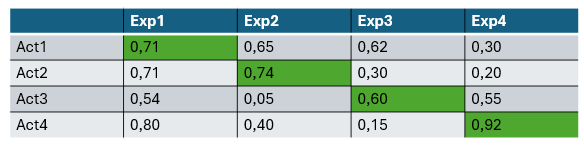
\includegraphics[width=0.60\textwidth]{assets/page_6_img_0.png}
\end{center}

\begin{center}
\begin{tabular}{lcccc}
\toprule
 & \textbf{Exp1} & \textbf{Exp2} & \textbf{Exp3} & \textbf{Exp4} \\
\midrule
\textbf{Act1} & \cellcolor{highlightgreen}\textbf{0.71} & 0.65 & 0.62 & 0.30 \\
\textbf{Act2} & 0.71 & \cellcolor{highlightgreen}\textbf{0.74} & 0.30 & 0.20 \\
\textbf{Act3} & 0.54 & 0.05 & \cellcolor{highlightgreen}\textbf{0.60} & 0.55 \\
\textbf{Act4} & 0.80 & 0.40 & 0.15 & \cellcolor{highlightgreen}\textbf{0.92} \\
\bottomrule
\end{tabular}
\end{center}

Which of the following thresholds is more dependable in terms of True Positive Rate (TPR) and False Positive Rate (FPR)?
\begin{center}
\textbf{Candidate Thresholds:} \quad $T = 0.70, \quad 0.80, \quad 0.90$
\end{center}
Provide full derivations of True Positives (TP), False Positives (FP), True Negatives (TN), False Negatives (FN), TPR, and FPR for each threshold, and justify your conclusion.
\end{questionbox}

% ------------------------------------------------------------------------------
% Question 10
% ------------------------------------------------------------------------------
\begin{questionbox}{Question 10 \hfill [1.00 Point $\vert$ Penalty: $-0.25$ Points per wrong selection]}
Which solutions can help address the challenge of variation in extracted requirements?
\begin{enumerate}[label=\alph*.,leftmargin=2em]
    \item Automatically rejecting extracted requirements with different phrasing
    \item Ignoring minor variations and focusing only on exact matches
    \item Using predefined synonym lists to map similar terms
    \item Using word embeddings to detect semantically similar words
    \item Manually reviewing every extracted requirement
\end{enumerate}
\end{questionbox}

% ------------------------------------------------------------------------------
% Question 11
% ------------------------------------------------------------------------------
\begin{questionbox}{Question 11 \hfill [1.50 Points $\vert$ Penalty: $-0.375$ Points]}
The following reward formulation can be used when fine-tuning a model on human feedback:
\begin{equation*}
    R(x, y) = r_\theta(x, y) - \beta \, \mathbb{D}_{\text{KL}}\left(\pi_\phi(y \mid x) \,\|\, \pi_{\text{ref}}(y \mid x)\right)
\end{equation*}
which can be expressed at the token or sequence level with the penalty term $-\beta \log \frac{\pi_\phi(y \mid x)}{\pi_{\text{ref}}(y \mid x)}$.\\
Here, $r_\theta(x, y)$ is the output of a Reward Model, and $\pi_\phi$ and $\pi_{\text{ref}}$ are the new and the original policies, respectively (representing the token probabilities assigned by the new and original models).\\
What is the purpose of the term $\log \frac{\pi_\phi(y \mid x)}{\pi_{\text{ref}}(y \mid x)}$?

\begin{enumerate}[label=\alph*.,leftmargin=2em]
    \item It increases the entropy of the output (i.e., it helps the model produce more ``creative'' answers)
    \item It improves the model's capability of following instructions
    \item It prevents the model from collapsing into a model that always predicts a single token
    \item It helps make the model more deterministic
    \item None of the other answers is correct
    \item It prevents the new model from producing outputs that are too dissimilar from the original one
    \item It rewards the model when it generates an answer that humans will ``like''
\end{enumerate}
\end{questionbox}

% ------------------------------------------------------------------------------
% Question 12
% ------------------------------------------------------------------------------
\begin{questionbox}{Question 12 \hfill [1.00 Point $\vert$ Penalty: $-0.25$ Points per wrong selection]}
What is ``priming'' in the context of prompt engineering?
\begin{enumerate}[label=\alph*.,leftmargin=2em]
    \item Using reinforcement learning to fine-tune the model
    \item Pre-training the model with additional data
    \item Providing initial input to guide the model's response
    \item Adding noise to the input to test model robustness
    \item Resetting the model before every new prompt
\end{enumerate}
\end{questionbox}

\newpage
% ==============================================================================
\section{Part II: Comprehensive Solutions \& In-Depth Analysis}
% ==============================================================================

% ------------------------------------------------------------------------------
% Solution 1
% ------------------------------------------------------------------------------
\begin{solutionbox}{Solution to Question 1: Debugging BERT Generation \& Encoder Limitations}
\textbf{Concise Exam Answer:}
\begin{quote}
\textbf{The code crashes with an \texttt{AttributeError} at Line 10 (\texttt{result = model.generate(**tokens)}).} \texttt{AutoModel} instantiates a bare \texttt{BertModel}, which lacks a generation head and does not implement \texttt{.generate()}. Furthermore, BERT is an encoder-only architecture trained bidirectionally on masked language modeling, not an autoregressive causal decoder capable of next-token generation.
\end{quote}

\subsubsection*{1. Runtime Mechanics and Exact Exception}
When executing the provided script:
\begin{lstlisting}[style=pythonstyle,numbers=none]
model = AutoModel.from_pretrained("bert-base-uncased")
...
result = model.generate(**tokens)
\end{lstlisting}
The Python runtime raises the following exception at Line 10:
\begin{lstlisting}[style=diffstyle]
AttributeError: 'BertModel' object has no attribute 'generate'
\end{lstlisting}
In the Hugging Face \texttt{transformers} library:
\begin{enumerate}
    \item \texttt{AutoModel.from\_pretrained(...)} loads the \emph{bare} base transformer backbone (specifically \texttt{BertModel}), which outputs contextual hidden state representations $\mathbf{H} \in \mathbb{R}^{B \times L \times d_{\text{model}}}$ from the final self-attention layer. It has no output vocabulary head (un-embedding matrix $W_U$) attached.
    \item The autoregressive generation API method \texttt{.generate()} is provided by the mixin class \texttt{GenerationMixin}. In Hugging Face, \texttt{GenerationMixin} is exclusively inherited by model classes equipped with language modeling heads, such as \texttt{AutoModelForCausalLM} (e.g., \texttt{GPT2LMHeadModel}, \texttt{LlamaForCausalLM}) or \texttt{AutoModelForSeq2SeqLM} (e.g., \texttt{T5ForConditionalGeneration}, \texttt{BartForConditionalGeneration}). Bare backbone models like \texttt{BertModel} do \emph{not} inherit from \texttt{GenerationMixin}.
\end{enumerate}

\subsubsection*{2. Architectural and Theoretical Foundations: Encoder vs. Causal Decoder}
Beyond the missing library method, the code snippet exhibits a fundamental conceptual mistake:
\begin{itemize}[leftmargin=1.5em]
    \item \textbf{Bidirectional Encoder Architecture (BERT):} BERT (Devlin et al., 2018) is an \emph{encoder-only} model. Its self-attention mechanism is entirely unmasked and bidirectional:
    \begin{equation}
        \mathbf{A}_{i,j} = \frac{\mathbf{q}_i^\top \mathbf{k}_j}{\sqrt{d_k}} \quad \forall i, j \in \{1, \dots, L\}
    \end{equation}
    Every token representation attends simultaneously to all prior and subsequent tokens in the sequence. BERT is pre-trained on \textbf{Masked Language Modeling (MLM)} and \textbf{Next Sentence Prediction (NSP)}. In MLM, $15\%$ of tokens are masked with \texttt{[MASK]} and predicted in parallel. BERT has no mechanism for step-by-step causal next-token sampling $P(w_t \mid w_{<t})$.
    
    \item \textbf{Autoregressive Causal Decoder (GPT / LLaMA):} Text generation requires an autoregressive decoder that enforces a lower-triangular causal attention mask:
    \begin{equation}
        \mathbf{M}_{i,j} = \begin{cases} 0 & \text{if } j \le i \\ -\infty & \text{if } j > i \end{cases}
    \end{equation}
    This ensures that token $w_t$ can only attend to past tokens $w_{<t}$, permitting valid probability factorizations $P(w_{1:T}) = \prod_{t=1}^T P(w_t \mid w_{<t})$ and token-by-token greedy or nucleus decoding.
\end{itemize}

\subsubsection*{3. How to Correct the Code}
If the developer's objective is open-ended sequence generation (e.g., completing ``The result of the operation 2 + 2 is ''), an autoregressive causal language model must be used:
\begin{lstlisting}[style=pythonstyle]
from transformers import AutoModelForCausalLM, AutoTokenizer
import torch

model_name = "gpt2" # or a causal LLaMA checkpoint
tokenizer = AutoTokenizer.from_pretrained(model_name)
model = AutoModelForCausalLM.from_pretrained(model_name)

prompt = "The result of the operation 2 + 2 is "
tokens = tokenizer(prompt, return_tensors="pt")

with torch.no_grad():
    output_tokens = model.generate(**tokens, max_new_tokens=10)
print(tokenizer.decode(output_tokens[0], skip_special_tokens=True))
\end{lstlisting}
If BERT was intended for Cloze token filling, one must instead use \texttt{AutoModelForMaskedLM} and supply a \texttt{[MASK]} token:
\begin{lstlisting}[style=pythonstyle]
from transformers import AutoModelForMaskedLM, AutoTokenizer
tokenizer = AutoTokenizer.from_pretrained("bert-base-uncased")
model = AutoModelForMaskedLM.from_pretrained("bert-base-uncased")
inputs = tokenizer("The result of the operation 2 + 2 is [MASK].", return_tensors="pt")
logits = model(**inputs).logits
mask_idx = (inputs.input_ids == tokenizer.mask_token_id).nonzero(as_tuple=True)[1]
predicted_token = tokenizer.decode(logits[0, mask_idx].argmax(dim=-1))
\end{lstlisting}
\end{solutionbox}

% ------------------------------------------------------------------------------
% Solution 2
% ------------------------------------------------------------------------------
\begin{solutionbox}{Solution to Question 2: Reflection Mechanisms in Agentic Architectures}
\textbf{Correct Choice:} \textbf{e} (``To evaluate past decisions and improve future performance'')

\subsubsection*{1. Theoretical Rationale \& Literature Context}
In agentic AI systems (e.g., \textsc{Reflexion} by Shinn et al., 2023; \textsc{Self-Refine} by Madaan et al., 2023; \textsc{ReAct} by Yao et al., 2022), \textbf{reflection} constitutes a metacognitive feedback loop. Rather than operating in an open-loop feed-forward manner (where an error irrevocably derails the task), an agent with reflection:
\begin{enumerate}
    \item \textbf{Evaluates Trajectories:} Analyzes execution feedback from the environment (e.g., unit test failures, compiler syntax errors, linter diagnostics, or human critiques).
    \item \textbf{Formulates Verbal Reflections:} Generates a semantic diagnosis of why the previous attempt failed and what specific tactical modifications are required.
    \item \textbf{Updates Memory:} Stores these synthesized reflections into episodic/working memory buffers, dynamically modifying the context for the next planning iteration.
\end{enumerate}
This iterative self-correction dramatically improves performance on complex reasoning, theorem proving, and automated software repair benchmarks (such as SWE-bench and HumanEval).

\subsubsection*{2. Detailed Breakdown of Distractors}
\begin{itemize}[leftmargin=1.5em]
    \item \textbf{Option a is incorrect:} Reflection does not eliminate structured workflows. On the contrary, reflection relies upon rigorous structural loops (such as Actor--Evaluator--Self-Reflection state machines).
    \item \textbf{Option b is incorrect:} Generating responses using predefined scripts describes rule-based chatterbots, which are rigid and antithetical to autonomous LLM reasoning.
    \item \textbf{Option c is incorrect:} This statement contains an oxymoron: ``store knowledge permanently in short-term memory''. Short-term memory (the active context window) is ephemeral; permanent storage occurs in external long-term vector databases.
    \item \textbf{Option d is incorrect:} Executing tasks without modifying strategies is the definition of non-adaptive execution. The foundational goal of reflection is specifically to adapt and revise failing strategies.
\end{itemize}
\end{solutionbox}

% ------------------------------------------------------------------------------
% Solution 3
% ------------------------------------------------------------------------------
\begin{solutionbox}{Solution to Question 3: Encoder Self-Attention vs. Cross-Attention}
\textbf{Correct Choice:} \textbf{g} (``Encoder self-attention only uses information from the input sequence, while encoder-decoder cross-attention allows the decoder to attend to the encoder's output'')

\subsubsection*{1. Mathematical Formulation}
The scaled dot-product attention operator across all Transformer modules is defined as:
\begin{equation}
    \text{Attention}(\mathbf{Q}, \mathbf{K}, \mathbf{V}) = \text{softmax}\left(\frac{\mathbf{Q} \mathbf{K}^\top}{\sqrt{d_k}}\right) \mathbf{V}
\end{equation}
The critical distinction lies in where the Query ($\mathbf{Q}$), Key ($\mathbf{K}$), and Value ($\mathbf{V}$) matrices originate:

\paragraph{Encoder Self-Attention:}
Let $\mathbf{X} \in \mathbb{R}^{n \times d_{\text{model}}}$ denote the input token representations (or hidden states from layer $l-1$ of the encoder). All three projections originate from the \emph{same} sequence:
\begin{equation}
    \mathbf{Q}_{\text{enc}} = \mathbf{X} \mathbf{W}_Q, \quad \mathbf{K}_{\text{enc}} = \mathbf{X} \mathbf{W}_K, \quad \mathbf{V}_{\text{enc}} = \mathbf{X} \mathbf{W}_V
\end{equation}
Every token in the input sequence computes attention over all other tokens in the input sequence bidirectionally. It operates strictly within the source domain.

\paragraph{Encoder-Decoder Cross-Attention:}
Let $\mathbf{S} \in \mathbb{R}^{m \times d_{\text{model}}}$ denote the decoder's intermediate representations (derived from the masked self-attention over previously generated target tokens), and let $\mathbf{H}_{\text{enc}} \in \mathbb{R}^{n \times d_{\text{model}}}$ denote the final output representations of the encoder stack. In cross-attention:
\begin{equation}
    \mathbf{Q}_{\text{cross}} = \mathbf{S} \mathbf{W}_Q, \quad \mathbf{K}_{\text{cross}} = \mathbf{H}_{\text{enc}} \mathbf{W}_K, \quad \mathbf{V}_{\text{cross}} = \mathbf{H}_{\text{enc}} \mathbf{W}_V
\end{equation}
Here, the decoder queries ($\mathbf{Q}$) probe the encoder's memory representations ($\mathbf{K}, \mathbf{V}$). This allows the generative decoder to condition its next token predictions on the complete semantic context of the input sequence.

\subsubsection*{2. Detailed Breakdown of Distractors}
\begin{itemize}[leftmargin=1.5em]
    \item \textbf{Option a is incorrect:} Cross-attention attends to the \emph{entire} input sequence (via all encoder key vectors $\mathbf{k}_1, \dots, \mathbf{k}_n$), not just a single ``current token''.
    \item \textbf{Option b is incorrect:} Inverts the mechanisms: encoder self-attention attends to prior encoder layers, while cross-attention attends to encoder outputs using decoder queries.
    \item \textbf{Option c is incorrect:} States that encoder self-attention occurs in the decoder, which is completely backwards.
    \item \textbf{Option d is incorrect:} Inverts the architectural locations of the blocks.
    \item \textbf{Option e is incorrect:} Because option (g) is strictly correct.
    \item \textbf{Option f is incorrect:} Attending to previous tokens in the output sequence is the function of \emph{masked decoder self-attention}, not cross-attention.
\end{itemize}
\end{solutionbox}

% ------------------------------------------------------------------------------
% Solution 4
% ------------------------------------------------------------------------------
\begin{solutionbox}{Solution to Question 4: Byte-Pair Encoding (BPE) Step-by-Step Derivation}
\textbf{Correct Formatted Answer:}
\begin{center}
\textbf{1st merge:} \texttt{a,a} \quad$\vert$\quad
\textbf{2nd merge:} \texttt{a,c} \quad$\vert$\quad
\textbf{3rd merge:} \texttt{ac,e}
\end{center}

\subsubsection*{1. Step-by-Step Mathematical Derivation}
Byte-Pair Encoding (Sennrich et al., 2016) is a greedy data compression algorithm adapted for subword tokenization. At each step, it identifies the most frequently co-occurring adjacent symbol pair across the corpus, merges them into a new single vocabulary symbol, and updates the tokenized sequence.

\paragraph{Initial State (Step 0):}
The initial sequence consists of 13 individual character tokens:
\begin{center}
\texttt{[a, c, e, a, c, e, a, a, a, a, a, c, b]}
\end{center}
Let us enumerate all adjacent symbol pairs and compute their frequencies:
\begin{itemize}[leftmargin=2em]
    \item Pair \texttt{('a', 'c')}: indices $(0,1)$, $(3,4)$, $(11,12) \implies$ \textbf{Frequency = 3}
    \item Pair \texttt{('c', 'e')}: indices $(1,2)$, $(4,5) \implies$ \textbf{Frequency = 2}
    \item Pair \texttt{('e', 'a')}: indices $(2,3)$, $(5,6) \implies$ \textbf{Frequency = 2}
    \item Pair \texttt{('a', 'a')}: in the sub-sequence \texttt{a a a a a} (indices 6 to 10), adjacent pairs appear at $(6,7), (7,8), (8,9), (9,10) \implies$ \textbf{Frequency = 4}
    \item Pair \texttt{('c', 'b')}: index $(11,12) \implies$ \textbf{Frequency = 1}
\end{itemize}
The maximum frequency is $\max = 4$, corresponding uniquely to the pair \texttt{('a', 'a')}.
\begin{takeawaybox}[Merge 1 Selection]
\textbf{1st merge:} \texttt{a,a} $\longrightarrow$ generates new token \texttt{aa}.
\end{takeawaybox}
Replacing all non-overlapping occurrences of \texttt{a a} from left to right in \texttt{a a a a a}:
\begin{itemize}
    \item Tokens at $6, 7 \to \texttt{aa}$
    \item Tokens at $8, 9 \to \texttt{aa}$
    \item Token at $10$ remains single \texttt{a}
\end{itemize}
Updated sequence after Merge 1 (11 tokens):
\begin{center}
\texttt{[a, c, e, a, c, e, aa, aa, a, c, b]}
\end{center}

\paragraph{State after Merge 1 (Step 1):}
Let us re-evaluate the frequencies of all adjacent pairs:
\begin{itemize}[leftmargin=2em]
    \item Pair \texttt{('a', 'c')}: indices $(0,1)$, $(3,4)$, and between the single \texttt{a} at index 8 and \texttt{c} at index 9: $(8,9) \implies$ \textbf{Frequency = 3}
    \item Pair \texttt{('c', 'e')}: indices $(1,2)$, $(4,5) \implies$ \textbf{Frequency = 2}
    \item Pair \texttt{('e', 'a')}: index $(2,3) \implies$ \textbf{Frequency = 1}
    \item Pair \texttt{('e', 'aa')}: index $(5,6) \implies$ \textbf{Frequency = 1}
    \item Pair \texttt{('aa', 'aa')}: index $(6,7) \implies$ \textbf{Frequency = 1}
    \item Pair \texttt{('aa', 'a')}: index $(7,8) \implies$ \textbf{Frequency = 1}
    \item Pair \texttt{('c', 'b')}: index $(9,10) \implies$ \textbf{Frequency = 1}
\end{itemize}
The most frequent adjacent pair is strictly \texttt{('a', 'c')} with frequency 3.
\begin{takeawaybox}[Merge 2 Selection]
\textbf{2nd merge:} \texttt{a,c} $\longrightarrow$ generates new token \texttt{ac}.
\end{takeawaybox}
Updated sequence after Merge 2 (8 tokens):
\begin{center}
\texttt{[ac, e, ac, e, aa, aa, ac, b]}
\end{center}

\paragraph{State after Merge 2 (Step 2):}
Let us re-evaluate the adjacent pair frequencies:
\begin{itemize}[leftmargin=2em]
    \item Pair \texttt{('ac', 'e')}: indices $(0,1)$ and $(2,3) \implies$ \textbf{Frequency = 2}
    \item Pair \texttt{('e', 'ac')}: index $(1,2) \implies$ \textbf{Frequency = 1}
    \item Pair \texttt{('e', 'aa')}: index $(3,4) \implies$ \textbf{Frequency = 1}
    \item Pair \texttt{('aa', 'aa')}: index $(4,5) \implies$ \textbf{Frequency = 1}
    \item Pair \texttt{('aa', 'ac')}: index $(5,6) \implies$ \textbf{Frequency = 1}
    \item Pair \texttt{('ac', 'b')}: index $(6,7) \implies$ \textbf{Frequency = 1}
\end{itemize}
The highest frequency is 2, corresponding uniquely to \texttt{('ac', 'e')}.
\begin{takeawaybox}[Merge 3 Selection]
\textbf{3rd merge:} \texttt{ac,e} $\longrightarrow$ generates new token \texttt{ace}.
\end{takeawaybox}
Final sequence after Merge 3 (6 tokens):
\begin{center}
\texttt{[ace, ace, aa, aa, ac, b]}
\end{center}
The three merged tokens produced, in exact sequential order, are \textbf{\texttt{a,a}}, \textbf{\texttt{a,c}}, and \textbf{\texttt{ac,e}}.
\end{solutionbox}

% ------------------------------------------------------------------------------
% Solution 5
% ------------------------------------------------------------------------------
\begin{solutionbox}{Solution to Question 5: Principles of BERTScore Evaluation}
\textbf{Correct Choice:} \textbf{g} (``It computes token-level similarity by aligning contextualized embeddings from a pre-trained transformer model and aggregating scores'')

\subsubsection*{1. Theoretical Rationale and Mathematical Formalism}
Traditional text generation metrics like BLEU and ROUGE rely on surface lexical $n$-gram matching. Consequently, they penalize semantically accurate paraphrases, synonyms, and reordered syntax. \textbf{BERTScore} (Zhang et al., ICLR 2020) solves this limitation by evaluating semantic similarity in continuous representation space:
\begin{enumerate}
    \item Given a candidate sentence $\hat{x} = \langle \hat{x}_1, \dots, \hat{x}_k \rangle$ and a reference sentence $x = \langle x_1, \dots, x_l \rangle$, BERTScore passes them through a pre-trained contextual transformer (e.g., RoBERTa, BERT) to extract contextualized token embeddings:
    \begin{equation}
        \mathbf{\hat{e}}_i = \frac{\text{BERT}(\hat{x})_i}{\|\text{BERT}(\hat{x})_i\|_2}, \qquad \mathbf{e}_j = \frac{\text{BERT}(x)_j}{\|\text{BERT}(x)_j\|_2}
    \end{equation}
    \item Pairwise cosine similarities between all tokens are computed: $S_{i,j} = \mathbf{\hat{e}}_i^\top \mathbf{e}_j$.
    \item Greedy bipartite matching is applied to compute \textbf{BERTScore Recall} and \textbf{Precision}:
    \begin{equation}
        R_{\text{BERT}} = \frac{1}{|x|} \sum_{x_j \in x} \max_{\hat{x}_i \in \hat{x}} \mathbf{\hat{e}}_i^\top \mathbf{e}_j, \qquad P_{\text{BERT}} = \frac{1}{|\hat{x}|} \sum_{\hat{x}_i \in \hat{x}} \max_{x_j \in x} \mathbf{\hat{e}}_i^\top \mathbf{e}_j
    \end{equation}
    \item The final metric is the harmonic mean: $F_{\text{BERT}} = 2 \frac{P_{\text{BERT}} \cdot R_{\text{BERT}}}{P_{\text{BERT}} + R_{\text{BERT}}}$.
\end{enumerate}

\subsubsection*{2. Detailed Breakdown of Distractors}
\begin{itemize}[leftmargin=1.5em]
    \item \textbf{Option a is incorrect:} Describes $n$-gram overlap metrics (like METEOR or tf-idf weighted BLEU), not BERTScore's contextualized vector alignment.
    \item \textbf{Option b is incorrect:} BERTScore does not use a fine-tuned binary classifier or cross-encoder; it utilizes frozen, pre-trained embeddings extracted from intermediate/final layers.
    \item \textbf{Option c is incorrect:} The candidate in the exam dump mistakenly selected this option. BERTScore does \emph{not} formulate evaluation as a masked language modeling fill-in-the-blank prompt.
    \item \textbf{Option d is incorrect:} BERTScore is entirely based on continuous vector dot-products; it does not construct or traverse discrete syntactic parse trees.
    \item \textbf{Option e is incorrect:} Static word embeddings (Word2Vec, GloVe) assign one fixed vector per word, completely failing to handle polysemy, syntactic role shifts, and contextual dependencies.
    \item \textbf{Option f is incorrect:} Bag-of-words ignores word ordering and context entirely.
\end{itemize}
\end{solutionbox}

% ------------------------------------------------------------------------------
% Solution 6
% ------------------------------------------------------------------------------
\begin{solutionbox}{Solution to Question 6: Absmax Quantization to int8}
\textbf{Correct Formatted Answer:}
\begin{align*}
    \text{quantized}(x_1) &= \mathbf{-127} \\
    \text{quantized}(x_2) &= \mathbf{102} \\
    \text{quantized}(x_3) &= \mathbf{-25} \\
    \text{quantized}(x_4) &= \mathbf{0}
\end{align*}

\subsubsection*{1. Mathematical Derivation of Symmetric Absmax Quantization}
In post-training quantization of LLM weights and activations (Dettmers et al., LLM.int8(), 2022), \textbf{absmax quantization} maps full-precision floating point numbers $X = \{x_1, \dots, x_N\}$ into signed 8-bit integers $\text{int8} \in [-127, 127]$ using a symmetric scale factor.

\paragraph{Step 1: Determine the Absolute Maximum ($x_{\text{max}}$):}
\begin{equation}
    x_{\text{max}} = \max_{i} |x_i| = \max(|-5|, |4|, |-1|, |0|) = \max(5, 4, 1, 0) = 5
\end{equation}

\paragraph{Step 2: Calculate the Quantization Scale Factor ($s$):}
For signed symmetric 8-bit integers with dynamic range $[-127, 127]$:
\begin{equation}
    s = \frac{q_{\text{max}}}{x_{\text{max}}} = \frac{127}{5} = 25.4
\end{equation}

\paragraph{Step 3: Quantize Each Value via Scaling and Rounding:}
The quantization formula is:
\begin{equation}
    q_i = \text{round}(s \cdot x_i) = \text{round}(25.4 \cdot x_i)
\end{equation}
Applying this to each input coordinate:
\begin{itemize}[leftmargin=2em]
    \item For $x_1 = -5$:
    \begin{equation*}
        q_1 = \text{round}(25.4 \times (-5)) = \text{round}(-127.0) = \mathbf{-127}
    \end{equation*}
    \item For $x_2 = 4$:
    \begin{equation*}
        q_2 = \text{round}(25.4 \times 4) = \text{round}(101.6) = \mathbf{102}
    \end{equation*}
    \item For $x_3 = -1$:
    \begin{equation*}
        q_3 = \text{round}(25.4 \times (-1)) = \text{round}(-25.4) = \mathbf{-25}
    \end{equation*}
    \item For $x_4 = 0$:
    \begin{equation*}
        q_4 = \text{round}(25.4 \times 0) = \text{round}(0.0) = \mathbf{0}
    \end{equation*}
\end{itemize}

\subsubsection*{2. Dequantization and Error Analysis}
To reconstruct the floating point approximation $\hat{x}_i$, the inverse transformation $\hat{x}_i = \frac{q_i}{s}$ is applied:
\begin{align*}
    \hat{x}_1 &= \frac{-127}{25.4} = -5.000 \quad (\text{Quantization error } = 0.000) \\
    \hat{x}_2 &= \frac{102}{25.4} \approx 4.0157 \quad (\text{Quantization error } = |4 - 4.0157| \approx 0.0157) \\
    \hat{x}_3 &= \frac{-25}{25.4} \approx -0.9843 \quad (\text{Quantization error } = |-1 - (-0.9843)| \approx 0.0157) \\
    \hat{x}_4 &= \frac{0}{25.4} = 0.000 \quad (\text{Quantization error } = 0.000)
\end{align*}
This achieves a $4\times$ memory reduction (from 32-bit floats to 8-bit integers) with negligible numerical degradation.
\end{solutionbox}

% ------------------------------------------------------------------------------
% Solution 7
% ------------------------------------------------------------------------------
\begin{solutionbox}{Solution to Question 7: Benefits of Open-Source Datasets}
\textbf{Correct Choices:} \textbf{a} and \textbf{c}
\begin{itemize}[leftmargin=1.5em]
    \item \textbf{a.} Authenticity and credibility of real-world data
    \item \textbf{c.} Ability to acquire timely data and share data freely
\end{itemize}

\subsubsection*{1. Theoretical Rationale}
\begin{itemize}[leftmargin=1.5em]
    \item \textbf{Authenticity of Real-World Data (Option a):} Open web crawls (e.g., Common Crawl, Wikipedia, GitHub, StackOverflow, RedPajama) reflect natural human language, diverse linguistic idioms, real-world software engineering paradigms, and actual domain-specific jargon that synthetic data often lacks.
    \item \textbf{Timely Acquisition and Free Sharing (Option c):} Open-source licensing permits public distribution, rapid community dissemination, collective auditing, academic reproducibility, and continuous updates as new libraries and software technologies emerge.
\end{itemize}

\subsubsection*{2. Detailed Breakdown of Distractors}
\begin{itemize}[leftmargin=1.5em]
    \item \textbf{Option b is false:} No dataset guarantees high model prediction accuracy. Accuracy depends on model parameter capacity, loss convergence, algorithmic design, data cleaning, and domain alignment. In fact, raw open-source web scrapes contain substantial noise, spam, and factual falsehoods.
    \item \textbf{Option d is false:} Open-source data extracted from the internet is notorious for containing historical, cultural, gender, and toxic societal biases. Openness does \emph{not} eliminate bias; rigorous deduplication, toxicity filtering, and alignment are mandatory.
    \item \textbf{Option e is false:} Pre-training on open-source text yields a foundational base model. Downstream task execution, instruction adherence, and safety guardrails strictly require supervised fine-tuning (SFT) and preference alignment (RLHF/DPO).
\end{itemize}
\end{solutionbox}

% ------------------------------------------------------------------------------
% Solution 8
% ------------------------------------------------------------------------------
\begin{solutionbox}{Solution to Question 8: Agentic Multi-Agent Architecture for Automated Code Generation and Iterative Test Refinement}
\subsubsection*{1. Critique of Candidate Submission in Raw Exam Dump}
In the recorded examination attempt, the student proposed an agent that ``tweaks the tests''. As the course examiner correctly annotated:
\begin{quote}
\textit{``The objective of the second agent would not be to tweak the tests but to refine the code to pass a set of stable test cases.''}
\end{quote}
In automated software engineering (LLM4SE), test cases constitute the formal specification and ground-truth acceptance oracle. Modifying tests to match buggy code destroys software reliability and violates verification guarantees. Below is the production-grade, theoretically sound agentic architecture.

\subsubsection*{2. System Architecture \& Workflow Pipeline}
The system implements a closed-loop iterative repair loop (analogous to \textsc{Reflexion} and \textsc{Self-Debugging}):
\begin{enumerate}
    \item \textbf{Code Generator Agent (Architect):} Receives natural language requirements (\texttt{REQS}) and test signatures, generating an initial candidate implementation $C_0$.
    \item \textbf{Deterministic Execution Sandbox (Tool Environment):} Executes $C_t$ against the immutable test suite \texttt{TESTS}. Returns execution status: either $\text{PASSED}$ (terminates pipeline) or $\text{FAILED}$ with structured failure logs (assertion messages, stack traces, stderr).
    \item \textbf{Code Refiner Agent (Debugger):} When tests fail, this agent analyzes the failing inputs, expected vs. actual outputs, and tracebacks. Using Chain-of-Thought (CoT) reasoning, it identifies the bug and outputs an updated implementation $C_{t+1}$.
    \item \textbf{Loop Controller:} Iterates until all tests pass or the maximum iteration budget ($T_{\text{max}} = 5$) is exhausted.
\end{enumerate}

\begin{center}
\begin{tcolorbox}[colback=white,colframe=secondary,arc=1mm,boxrule=0.6pt,width=0.95\textwidth]
\small\centering
\textbf{Closed-Loop Agentic Flow:}\\
$\texttt{REQS} \longrightarrow \text{Code Generator} \xrightarrow{C_0} \text{Sandbox} \xrightarrow[\text{Failures}]{\text{Tracebacks}} \text{Code Refiner} \xrightarrow{C_{t+1}} \text{Sandbox} \xrightarrow[\text{All Pass}]{\text{Success}} \text{Verified Code}$
\end{tcolorbox}
\end{center}

\subsubsection*{3. Comprehensive Specification for Agent 1: Code Generator Agent}
\begin{itemize}[leftmargin=1.5em]
    \item \textbf{Role in Pipeline:} Analyzes the requirements specification \texttt{REQS} and produces a syntactically correct, self-contained Python implementation of the target function.
    \item \textbf{System Message:}
\begin{lstlisting}[style=diffstyle]
You are an expert Python Software Engineer. Your role is to generate clean, robust, and PEP-8 compliant code implementing the exact functionality specified in the provided requirements. You must return only the complete Python function enclosed in ```python ... ``` blocks, with no conversational filler.
\end{lstlisting}
    \item \textbf{Context:} The natural language functional requirements (\texttt{REQS}) and the test case signatures/specifications (\texttt{TESTS}).
    \item \textbf{Possible Inputs:}
\begin{lstlisting}[style=diffstyle]
REQS: "Implement a function `parse_version(v: str) -> tuple` that parses a semantic version string (e.g. '1.10.2') into a tuple of integers. It must handle pre-release tags by ignoring any suffix after a hyphen."
TESTS: [
  {"input": "'1.2.3'", "expected": "(1, 2, 3)"},
  {"input": "'2.0.0-alpha'", "expected": "(2, 0, 0)"}
]
\end{lstlisting}
    \item \textbf{Expected Output:}
\begin{lstlisting}[style=diffstyle]
```python
def parse_version(v: str) -> tuple:
    clean_v = v.split('-')[0]
    return tuple(int(x) for x in clean_v.split('.'))
```
\end{lstlisting}
\end{itemize}

\subsubsection*{4. Comprehensive Specification for Agent 2: Code Refiner Agent}
\begin{itemize}[leftmargin=1.5em]
    \item \textbf{Role in Pipeline:} Acts as an automated debugger. It evaluates the current buggy implementation alongside failing test traces, identifies the root semantic bug, and synthesizes a corrected implementation without regressing passing tests.
    \item \textbf{System Message:}
\begin{lstlisting}[style=diffstyle]
You are an expert Automated Program Repair (APR) agent. You are given a function requirement, the current candidate code, and detailed execution feedback showing failing test cases.
Analyze the bug step-by-step:
1. Explain why the current implementation failed on the failing test cases.
2. Formulate the precise algorithmic fix required.
3. Output the fully corrected, complete replacement function inside ```python ... ``` blocks.
Never alter or complain about the test cases; they are ground truth.
\end{lstlisting}
    \item \textbf{Context:} Original requirements \texttt{REQS}, immutable test suite \texttt{TESTS}, current implementation $C_t$, and full execution traceback logs from the deterministic sandbox.
    \item \textbf{Possible Inputs:}
\begin{lstlisting}[style=diffstyle]
CURRENT_CODE:
def parse_version(v: str) -> tuple:
    return tuple(int(x) for x in v.split('.'))

EXECUTION_LOGS:
Test 1 ('1.2.3'): PASSED
Test 2 ('2.0.0-alpha'): FAILED -> ValueError: invalid literal for int() with base 10: '0-alpha'
\end{lstlisting}
    \item \textbf{Expected Output:}
\begin{lstlisting}[style=diffstyle]
### Root Cause Analysis:
The function splits the input directly by '.' without stripping optional pre-release suffixes denoted by '-'. Consequently, '0-alpha' cannot be cast to an integer.

### Corrected Code:
```python
def parse_version(v: str) -> tuple:
    base_version = v.split('-')[0]
    return tuple(int(part) for part in base_version.split('.'))
```
\end{lstlisting}
\end{itemize}
\end{solutionbox}

% ------------------------------------------------------------------------------
% Solution 9
% ------------------------------------------------------------------------------
\begin{solutionbox}{Solution to Question 9: Similarity Matrix, Threshold Optimization, and ROC Analysis}
\textbf{Correct Answer:} \textbf{The threshold $T = 0.70$ is the most dependable threshold.}

\subsubsection*{1. Problem Setup and Ground-Truth Identification}
We are given a $4 \times 4$ similarity matrix evaluated across 4 actual artifacts (\texttt{Act1}--\texttt{Act4}) and 4 expected artifacts (\texttt{Exp1}--\texttt{Exp4}), representing a total of $4 \times 4 = 16$ candidate trace links.
\begin{center}
\begin{tabular}{lcccc}
\toprule
 & \textbf{Exp1} & \textbf{Exp2} & \textbf{Exp3} & \textbf{Exp4} \\
\midrule
\textbf{Act1} & \cellcolor{highlightgreen}\textbf{0.71} & 0.65 & 0.62 & 0.30 \\
\textbf{Act2} & 0.71 & \cellcolor{highlightgreen}\textbf{0.74} & 0.30 & 0.20 \\
\textbf{Act3} & 0.54 & 0.05 & \cellcolor{highlightgreen}\textbf{0.60} & 0.55 \\
\textbf{Act4} & 0.80 & 0.40 & 0.15 & \cellcolor{highlightgreen}\textbf{0.92} \\
\bottomrule
\end{tabular}
\end{center}

\paragraph{Ground-Truth Partitioning:}
\begin{itemize}[leftmargin=1.5em]
    \item \textbf{True Positives Class ($P = 4$):} The diagonal elements (highlighted green in the exam figure) represent the valid ground-truth trace links:
    \begin{align*}
        \mathcal{P} = \{ &(\text{Act1},\text{Exp1})=0.71, \; (\text{Act2},\text{Exp2})=0.74, \\
                         &(\text{Act3},\text{Exp3})=0.60, \; (\text{Act4},\text{Exp4})=0.92 \}
    \end{align*}
    \item \textbf{True Negatives Class ($N = 12$):} The remaining 12 off-diagonal elements represent non-matching artifact pairs:
    \begin{align*}
        \mathcal{N} = \{ & 0.65, \, 0.62, \, 0.30, \quad (\text{Row 1}) \\
                         & 0.71, \, 0.30, \, 0.20, \quad (\text{Row 2}) \\
                         & 0.54, \, 0.05, \, 0.55, \quad (\text{Row 3}) \\
                         & 0.80, \, 0.40, \, 0.15 \quad (\text{Row 4}) \}
    \end{align*}
    Note that the universe of links is $|\mathcal{P}| + |\mathcal{N}| = 4 + 12 = 16$.
\end{itemize}

\paragraph{Classification Metric Definitions:}
For a similarity threshold $T$, a candidate link is predicted positive if $\text{sim} \ge T$, and negative otherwise:
\begin{equation}
    \text{TPR} = \frac{\text{TP}}{P} = \frac{\text{TP}}{\text{TP} + \text{FN}}, \qquad \text{FPR} = \frac{\text{FP}}{N} = \frac{\text{FP}}{\text{FP} + \text{TN}}
\end{equation}

\subsubsection*{2. Step-by-Step Derivations for Each Threshold}

\paragraph{Case 1: Threshold $T = 0.70$}
\begin{itemize}[leftmargin=1.5em]
    \item \textbf{Evaluating Positives ($\mathcal{P}$):}
    \begin{itemize}
        \item $(\text{Act1}, \text{Exp1}) = 0.71 \ge 0.70 \implies \text{TP}$
        \item $(\text{Act2}, \text{Exp2}) = 0.74 \ge 0.70 \implies \text{TP}$
        \item $(\text{Act3}, \text{Exp3}) = 0.60 < 0.70 \implies \text{FN}$
        \item $(\text{Act4}, \text{Exp4}) = 0.92 \ge 0.70 \implies \text{TP}$
    \end{itemize}
    $\implies \mathbf{TP = 3}, \quad \mathbf{FN = 1} \quad (TP + FN = 4)$.
    \begin{equation*}
        \mathbf{TPR} = \frac{3}{4} = \mathbf{0.75} \quad (75.0\%)
    \end{equation*}

    \item \textbf{Evaluating Negatives ($\mathcal{N}$):}
    Pairs with similarity $\ge 0.70$:
    \begin{itemize}
        \item $(\text{Act2}, \text{Exp1}) = 0.71 \ge 0.70 \implies \text{FP}$
        \item $(\text{Act4}, \text{Exp1}) = 0.80 \ge 0.70 \implies \text{FP}$
    \end{itemize}
    All other 10 off-diagonal values are strictly below 0.70 ($0.65, 0.62, 0.30, 0.30, 0.20, 0.54, 0.05, 0.55, 0.40, 0.15$).
    $\implies \mathbf{FP = 2}, \quad \mathbf{TN = 10} \quad (FP + TN = 12)$.
    \begin{equation*}
        \mathbf{FPR} = \frac{2}{12} = \frac{1}{6} \approx \mathbf{0.1667} \quad (16.67\%)
    \end{equation*}
\end{itemize}

\paragraph{Case 2: Threshold $T = 0.80$}
\begin{itemize}[leftmargin=1.5em]
    \item \textbf{Evaluating Positives ($\mathcal{P}$):}
    Only $(\text{Act4}, \text{Exp4}) = 0.92 \ge 0.80$. The remaining three ($0.71, 0.74, 0.60$) are $< 0.80$.
    $\implies \mathbf{TP = 1}, \quad \mathbf{FN = 3}$.
    \begin{equation*}
        \mathbf{TPR} = \frac{1}{4} = \mathbf{0.25} \quad (25.0\%)
    \end{equation*}

    \item \textbf{Evaluating Negatives ($\mathcal{N}$):}
    Among the 12 negative pairs, only $(\text{Act4}, \text{Exp1}) = 0.80 \ge 0.80 \implies \text{FP}$. The other 11 values are $< 0.80$.
    $\implies \mathbf{FP = 1}, \quad \mathbf{TN = 11}$.
    \begin{equation*}
        \mathbf{FPR} = \frac{1}{12} \approx \mathbf{0.0833} \quad (8.33\%)
    \end{equation*}
    \textit{(Note: If strict inequality $\text{sim} > 0.80$ is assumed, $\text{FP}=0, \text{TN}=12 \implies \text{FPR}=0$, but TPR remains unacceptably low at $0.25$).}
\end{itemize}

\paragraph{Case 3: Threshold $T = 0.90$}
\begin{itemize}[leftmargin=1.5em]
    \item \textbf{Evaluating Positives ($\mathcal{P}$):}
    Only $(\text{Act4}, \text{Exp4}) = 0.92 \ge 0.90 \implies \mathbf{TP = 1}, \quad \mathbf{FN = 3}$.
    \begin{equation*}
        \mathbf{TPR} = \frac{1}{4} = \mathbf{0.25} \quad (25.0\%)
    \end{equation*}
    \item \textbf{Evaluating Negatives ($\mathcal{N}$):}
    No off-diagonal element satisfies $\text{sim} \ge 0.90$ (the maximum off-diagonal value is 0.80).
    $\implies \mathbf{FP = 0}, \quad \mathbf{TN = 12}$.
    \begin{equation*}
        \mathbf{FPR} = \frac{0}{12} = \mathbf{0.00} \quad (0.0\%)
    \end{equation*}
\end{itemize}

\subsubsection*{3. Comprehensive Synthesis \& Dependability Justification}
\begin{center}
\small
\begin{tabular}{lcccccccc}
\toprule
\textbf{Threshold ($T$)} & \textbf{TP} & \textbf{FP} & \textbf{TN} & \textbf{FN} & \textbf{TPR (Recall)} & \textbf{FPR} & \textbf{Precision} & \textbf{$F_1$-Score} \\
\midrule
$\mathbf{T = 0.70}$ & \textbf{3} & \textbf{2} & \textbf{10} & \textbf{1} & $\mathbf{0.750}$ & $\mathbf{0.167}$ & $\mathbf{0.600}$ & $\mathbf{0.667}$ \\
$T = 0.80$          & 1          & 1          & 11          & 3          & $0.250$          & $0.083$          & $0.500$          & $0.333$ \\
$T = 0.90$          & 1          & 0          & 12          & 3          & $0.250$          & $0.000$          & $1.000$          & $0.400$ \\
\bottomrule
\end{tabular}
\end{center}

\paragraph{Why $T = 0.70$ is the most dependable:}
\begin{enumerate}
    \item \textbf{Asymmetry of Costs in Requirements Traceability:} In software engineering verification and trace link recovery, a \textbf{False Negative} (missed link) means an architectural component or unit test is completely detached from its functional requirement, leading to undetected compliance failures or untested safety critical functions. Conversely, a \textbf{False Positive} merely incurs a minor human verification cost.
    \item \textbf{Catastrophic Recall Degradation at Higher Thresholds:} Increasing $T$ from $0.70$ to $0.80$ drops the True Positive Rate from $75\%$ to an abysmal $25\%$ (missing 3 out of 4 requirements links).
    \item \textbf{Optimal Balance on ROC Curve:} At $T = 0.70$, the model achieves a high TPR of $0.75$ while bounding the False Positive Rate to a modest $16.7\%$ ($2$ false alarms out of $12$ negative links). It achieves the highest $F_1$-score ($0.667$).
\end{enumerate}

\paragraph{Examiner Note on Student Derivation in Raw Exam Dump:}
The candidate in the raw exam scored only 1.00/2.00 because while their final selection ($T=0.70$) was correct, their intermediate calculations contained critical errors:
\begin{itemize}
    \item At $T=0.70$, the student wrote $TP=3, FN=2 \implies TPR = 3/5 = 0.6$ and $TN=10, FP=1 \implies FPR = 1/11 = 0.09$. The candidate hallucinated 5 positive links instead of 4 and missed an off-diagonal FP.
    \item At $T=0.80$, the student wrote $TP=1, FN=0 \implies TPR = 1/1 = 1.0$, which is mathematically absurd since 3 positive links fell below the 0.80 threshold.
\end{itemize}
\end{solutionbox}

% ------------------------------------------------------------------------------
% Solution 10
% ------------------------------------------------------------------------------
\begin{solutionbox}{Solution to Question 10: Mitigating Linguistic Variation in Requirements}
\textbf{Correct Choices:} \textbf{c} and \textbf{d}
\begin{itemize}[leftmargin=1.5em]
    \item \textbf{c.} Using predefined synonym lists to map similar terms
    \item \textbf{d.} Using word embeddings to detect semantically similar words
\end{itemize}

\subsubsection*{1. Theoretical Rationale}
In Natural Language Requirements Engineering (NLRE), the \textbf{vocabulary mismatch problem} arises because different stakeholders, systems, and specifications express identical functional behaviors using disparate terminology (e.g., ``user'', ``client'', ``subscriber''; or ``terminate'', ``abort'', ``cancel''). Two effective AI/NLP strategies resolve this ambiguity:
\begin{itemize}[leftmargin=1.5em]
    \item \textbf{Controlled Ontologies and Synonym Lists (Option c):} Using curated domain dictionaries or WordNet synsets allows automated pipelines to canonicalize disparate surface tokens to a standardized root concept.
    \item \textbf{Dense Word / Sentence Embeddings (Option d):} Continuous representation models (Word2Vec, GloVe, Sentence-BERT) embed lexical items into high-dimensional geometric spaces where semantic relatedness corresponds to vector proximity (high cosine similarity), enabling soft semantic matching that bridges synonymy and paraphrasing.
\end{itemize}

\subsubsection*{2. Detailed Breakdown of Distractors}
\begin{itemize}[leftmargin=1.5em]
    \item \textbf{Option a is incorrect:} Automatically rejecting requirements due to differing phrasing would discard valid stakeholder requirements, catastrophically reducing system recall.
    \item \textbf{Option b is incorrect:} Requiring exact lexical matches is brittle and fails completely on natural language variation.
    \item \textbf{Option e is incorrect:} Requiring manual human review for every requirement defeats the entire purpose of automated NLP extraction and does not scale to large software architectures.
\end{itemize}
\end{solutionbox}

% ------------------------------------------------------------------------------
% Solution 11
% ------------------------------------------------------------------------------
\begin{solutionbox}{Solution to Question 11: The KL Divergence Regularizer in RLHF}
\textbf{Correct Choice:} \textbf{f} (``It prevents the new model from producing outputs that are too dissimilar from the original one'')

\subsubsection*{1. Mathematical Derivation of the RLHF Objective}
In Reinforcement Learning from Human Feedback (RLHF) via Proximal Policy Optimization (PPO; Ziegler et al., 2019; Ouyang et al., InstructGPT, 2022), the policy $\pi_\phi$ is optimized against an empirical reward model $r_\theta(x, y)$ subject to a Kullback-Leibler (KL) divergence penalty against the frozen supervised fine-tuned (SFT) reference policy $\pi_{\text{ref}}$:
\begin{equation}
    \max_\phi \; \mathbb{E}_{x \sim \mathcal{D}, \, y \sim \pi_\phi(\cdot \mid x)} \left[ r_\theta(x, y) - \beta \, \mathbb{D}_{\text{KL}}\left(\pi_\phi(y \mid x) \,\|\, \pi_{\text{ref}}(y \mid x)\right) \right]
\end{equation}
Expanding the KL divergence for a discrete output sequence $y$:
\begin{equation}
    \mathbb{D}_{\text{KL}}\left(\pi_\phi(y \mid x) \,\|\, \pi_{\text{ref}}(y \mid x)\right) = \sum_{t=1}^{|y|} \log \frac{\pi_\phi(y_t \mid x, y_{<t})}{\pi_{\text{ref}}(y_t \mid x, y_{<t})}
\end{equation}
The penalty term $-\beta \log \frac{\pi_\phi}{\pi_{\text{ref}}}$ penalizes policy updates whenever $\pi_\phi$ places significantly higher probability mass on tokens than the original model $\pi_{\text{ref}}$.

\subsubsection*{2. Theoretical Necessity: Mitigating Reward Hacking and Policy Drift}
\begin{enumerate}
    \item \textbf{Preventing Reward Model Exploitation (Reward Hacking):} The reward model $r_\theta$ is a learned proxy and imperfect approximation of human judgment. In high-dimensional optimization, an unconstrained policy quickly discovers adversarial vulnerabilities or degenerate sequences (e.g., repetitive punctuation or specific buzzwords) that achieve artificially high reward scores despite being nonsensical to humans (Goodhart's Law).
    \item \textbf{Preventing Policy Collapse and Drift:} The KL regularizer anchors the policy to the distribution of natural, grammatically correct language learned during pre-training and SFT, preserving core reasoning and linguistic fluency.
\end{enumerate}

\subsubsection*{3. Detailed Breakdown of Distractors}
\begin{itemize}[leftmargin=1.5em]
    \item \textbf{Option a is incorrect:} Policy entropy is governed by the entropy bonus $\mathcal{H}(\pi) = -\sum \pi \log \pi$. The KL divergence constrains the policy toward $\pi_{\text{ref}}$, which reduces rather than increases ungrounded randomness.
    \item \textbf{Option b is incorrect:} Instruction following capability is imparted by supervised instruction tuning (SFT) and the reward model scoring, not specifically by penalizing divergence from $\pi_{\text{ref}}$.
    \item \textbf{Option c is incorrect:} Preventing mode collapse to a single token is handled by sampling temperatures and entropy bonuses.
    \item \textbf{Option d is incorrect:} The KL penalty does not make generation deterministic; decoding strategies (greedy vs. nucleus sampling) control determinism.
    \item \textbf{Option e is incorrect:} The candidate in the exam dump mistakenly selected this option. Option (f) is the precise theoretical definition.
    \item \textbf{Option g is incorrect:} Rewarding human preference is the explicit responsibility of the primary reward term $r_\theta(x, y)$, whereas the log-ratio acts as a subtrahend penalty.
\end{itemize}
\end{solutionbox}

% ------------------------------------------------------------------------------
% Solution 12
% ------------------------------------------------------------------------------
\begin{solutionbox}{Solution to Question 12: Priming in Prompt Engineering}
\textbf{Correct Choice:} \textbf{c} (``Providing initial input to guide the model's response'')

\subsubsection*{1. Theoretical Rationale \& Cognitive Context}
In prompt engineering and cognitive psychology applied to generative AI, \textbf{priming} refers to the deliberate technique of prepending contextual cues, persona roles, stylistic exemplars, or conceptual prefaces at the beginning of the prompt context window.
\begin{itemize}[leftmargin=1.5em]
    \item \textbf{Attention Conditioning:} By introducing specific semantic tokens into the prefix (e.g., ``You are a senior security auditor analyzing C code for buffer overflows''), the multi-head self-attention mechanism activates specialized latent subspaces and associations learned during pre-training.
    \item \textbf{Steering Probability Trajectories:} Priming shifts the conditional probability distribution $P(w_t \mid w_{<t})$ toward relevant vocabulary, desired formality levels, and specific domain paradigms before the primary user query is processed.
\end{itemize}

\subsubsection*{2. Detailed Breakdown of Distractors}
\begin{itemize}[leftmargin=1.5em]
    \item \textbf{Option a is incorrect:} Reinforcement learning (e.g., PPO, DPO) modifies model weights through gradient descent during the post-training phase, which is fundamentally distinct from in-context prompt engineering.
    \item \textbf{Option b is incorrect:} Pre-training with additional data refers to continuous pre-training / domain-adaptive pre-training (DAPT).
    \item \textbf{Option d is incorrect:} Adding noise describes adversarial perturbation, stress-testing, or data augmentation.
    \item \textbf{Option e is incorrect:} Clearing or resetting model conversational state is context management, not semantic priming.
\end{itemize}
\end{solutionbox}

\end{document}
